% CVPR 2022 Paper Template
% based on the CVPR template provided by Ming-Ming Cheng (https://github.com/MCG-NKU/CVPR_Template)
% modified and extended by Stefan Roth (stefan.roth@NOSPAMtu-darmstadt.de)

\documentclass[10pt,twocolumn,letterpaper]{article}

%%%%%%%%% PAPER TYPE  - PLEASE UPDATE FOR FINAL VERSION
% \usepackage[review]{cvpr}      % To produce the REVIEW version
\usepackage{cvpr}              % To produce the CAMERA-READY version
%\usepackage[pagenumbers]{cvpr} % To force page numbers

\usepackage{graphicx}
\graphicspath{ {./image/} }
\usepackage{caption}
\usepackage{subcaption}
\usepackage{graphicx}
\usepackage{amsmath}
\usepackage{amssymb}
\usepackage{booktabs}
\usepackage{listings}
\usepackage{color}
\usepackage{ragged2e}
\usepackage[pagebackref,breaklinks,colorlinks]{hyperref}

% Support for easy cross-referencing
\usepackage[capitalize]{cleveref}
\crefname{section}{Sec.}{Secs.}
\Crefname{section}{Section}{Sections}
\Crefname{table}{Table}{Tables}
\crefname{table}{Tab.}{Tabs.}

%%%%%%%%% PAPER ID  - PLEASE UPDATE
\def\cvprPaperID{918299101} % *** Enter the CVPR Paper ID here
\def\confName{CVPR}
\def\confYear{2023}

\newcommand{\referencelink}[3]{\raggedright #1. \url{#2}. Accessed: #3.}

\begin{document}

%%%%%%%%% TITLE - PLEASE UPDATE
\title{Acquiring, Processing, and Displaying JWST NIRCam Imaging Data}
\cvprfinaltrue

\author{Maxwell Oakes\\
Portland State University\\
1900 SW 4th Ave, Portland, OR 97201\\
{\tt\small maxoakes@pdx.edu}}
\maketitle

%%%%%%%%% ABSTRACT
\begin{abstract}
  Images coming back from the James Webb Space Telescope (JWST) present a fascinating and awe-inspiring look at distant celestial objects and provide a glimpse at the early history of the universe. 
  This paper provides an overview of JWST and its mission, then summarizes the steps taken to replicate the manual work that is done in order to convert the raw astronomical imaging data into the vivid RGB images that have been released by the National Aeronautics and Space Administration (NASA). 
  Also in this paper, methods to acquire the image files via download will be addressed, as well as an overview of the FITS file format in which they are contained.
  The method used in this project to align the images will be explained, and alternative methods of doing this will also be discussed. The steps taken to assign color and combine the images will also be reviewed.
  The color images released publicly by NASA from JWST are processed manually by artists that have already spent much time in the field. While this project does automate some steps in the coloring and alignment process, there is a subjective element that may always continue to elude any automatic pipeline for this process.
\end{abstract}

%%%%%%%%% BODY TEXT
\section{Introduction}
\label{sec:intro}

The James Webb Space Telescope (JWST) was launched December 25th, 2021 as a successor to Hubble Space Telescope. The mission for JWST is to examine every phase of cosmic history; ranging from the first stars after the Big Bang to the formation of galaxies, stars and planets. Of the goals for JWST, there are four themes: 
(1) peer back in time with infrared imaging to see the formation of the first stars and galaxies, 
(2) use highly-sensitive infrared technology to view faint and early galaxies to help us understand how they are formed,
(3) see through clouds of dust and gas to observe how planetary systems are born
and (4) study atmospheres of extrasolar planets in hopes of finding the building blocks of life elsewhere in the universe, as well as within our own solar system \cite{webbobjective}.
Altogether, these objectives aim to give humanity a better understanding of the universe and its formation, and help us better understand our place in the universe.

Being able to meaningfully process data from JWST will prove to be immensely important in achieving these objectives. Additionally, allowing the public audience to see the fruits of JWST will drive fascination, and perhaps garner support in its ultimate objective.

Currently, the publishing of images from JWST's NIRCam imager requires a mix of computer science and art to achieve eye-catching imagery, often requiring external photo editing software and subjective judgement to make the best decisions.

This project aims to streamline the post-processing step of NIRCam data by automatically downloading imaging data from Space Telescope Science Institute's (STSI) MAST public archive, select the best wavelength-filtered exposure images and combine them into a single correctly-aligned, 8-bit RGB color image.

\section{Background Information}
\label{sec:background}

The following offers a short description of JWST and its instruments and capabilities, and gives a summary of the processing pipeline of imaging data, and concludes with the basic data structure that this imaging data comes in.

\subsection{Onboard Instruments}

\begin{figure*}
  \centering
    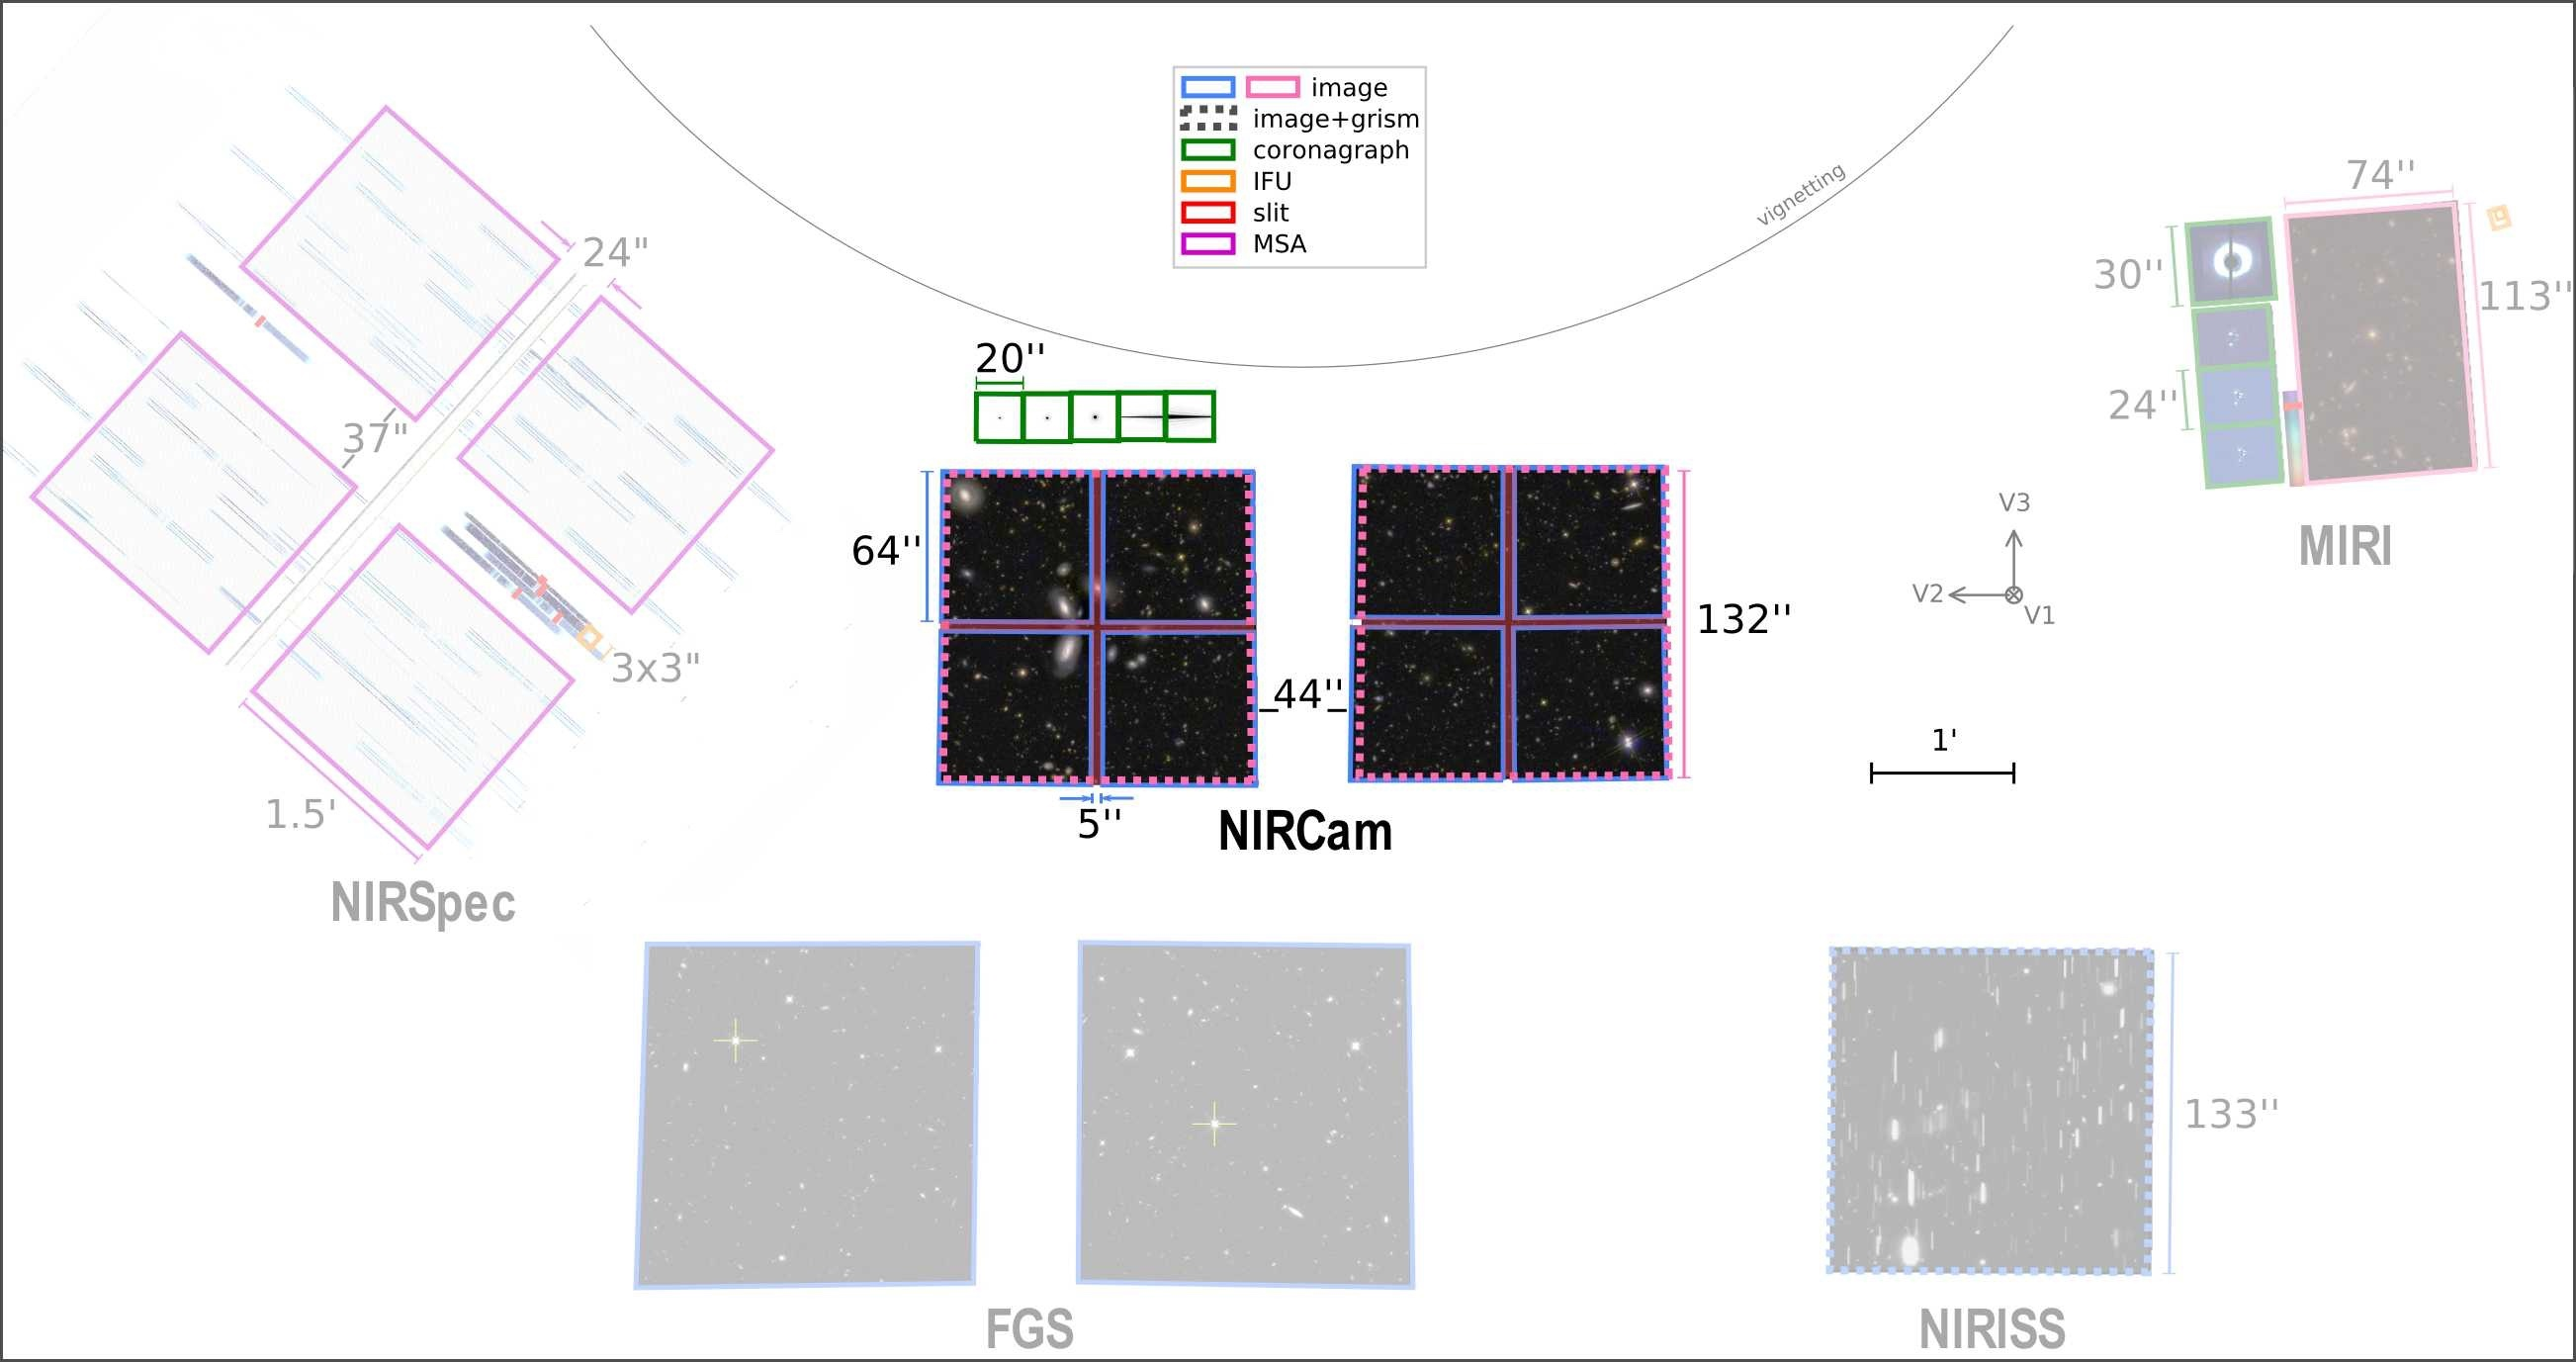
\includegraphics[scale=0.18]{instrument_array}
  \caption{Placement of the instrument array onboard JWST \cite{webbnircam}. The instrument that is focused is NIRCam, the primary tool that will be used in the project presented in this paper.}
  \label{fig:instruments}
\end{figure*}

In order to achieve JWST's objectives, the telescope is armed with several imaging and spectroscopy tools described below, and shown in \cref{fig:instruments}:
\newline
\textbf{MIRI Imager:} A camera sensor able to capture light with wavelengths between $5.6 - 25.5\mu m$. It offers 9 broadband filters allowing the capture of smaller portions of this light bandwidth. 
The camera itself has a field of view of $74'' \times 113''$. It also features several dither patterns that improve sampling at the shorter wavelengths, and remove artifacts from the detector or cosmic ray hits \cite{webbmiri}.
\newline
\textbf{NIRCam Infrared Camera:} A tool that offers many observation modes from regular imaging to coronagraphic imaging, to wide field slitless spectroscopy. For this project, NIRCam will be the primary instrument that is studied and utilized.
For imaging, NIRCam captures two $2.2' \times 2.2'$ fields that cover $9.7$ arcmin$^2$ with a total of 29 available wavelength filters.
The coronagraphic imaging mode offers round and bar-shaped occulting masks allowing for the capture of a star's corona without capturing the intense light of the star's center \cite{webbnircam}. In some of the images shown in this paper, some of the larger stars will occlusion masks covering them.
\newline
\textbf{NIRISS Imaging:} An imager that enables capture of wavelengths between $0.8 - 5.0\mu m$ in a $2.2' \times 2.2'$ field of view. 
Like NIRCam, NIRISS offers spectroscopy, but it is more sensitive to low surface brightness between $0.8$ and $2.5\mu m$. 
NIRISS imaging is also an alternative to NIRCam in cases where the position of a target is not known with great accuracy \cite{webbniriss}.
\newline
\textbf{NIRSPEC Spectroscopy:} Provides near-IR spectroscopy between $0.6 - 5.3 \mu m$ in a $3.4 \times 3.6$ arcmin field of view. It is designed to be especially powerful for multiplexing spectroscopy and high-contrast, high-throughput single-object spectroscopy \cite{webbnirspec}.

\subsection{Filters}

\begin{figure}[t]
  \centering
  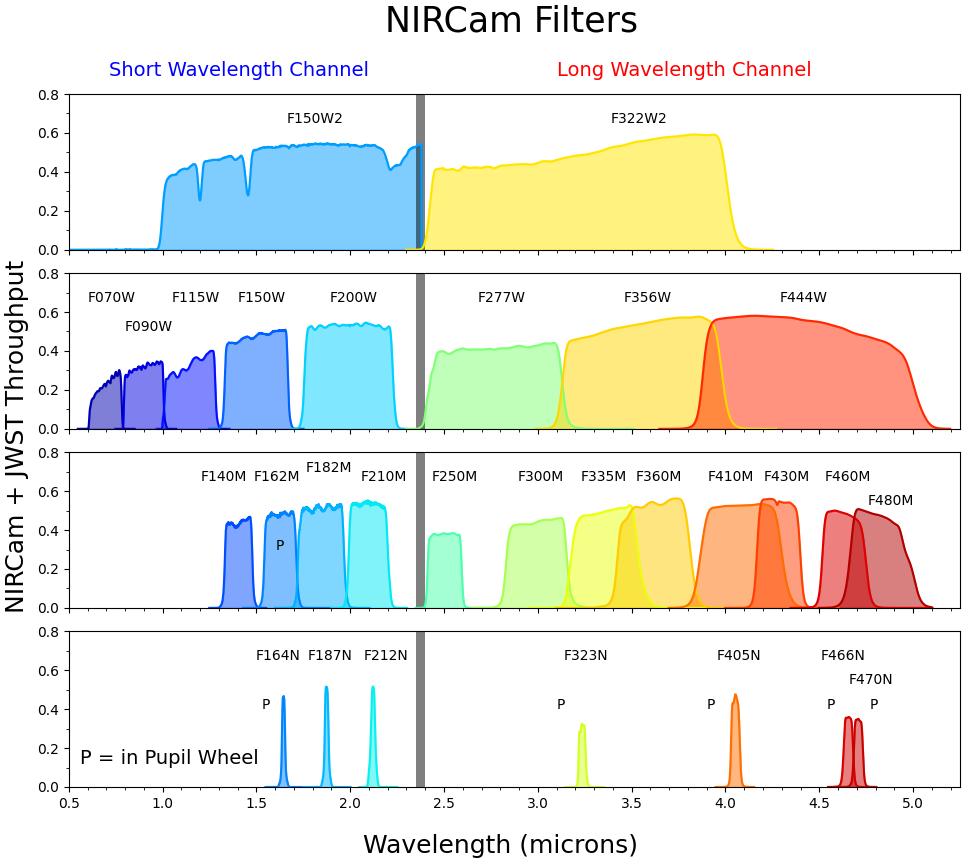
\includegraphics[scale=0.33]{filters}
  \caption{Available filters for the NIRCam instrument. Those marked with (P) are on the pupil wheel which require transmission through a second filter on the filter wheel \cite{webbfilters}.}
  \label{fig:filters}
\end{figure}

JWST is able to capture between $0.6 - 28.8\mu m$ over all available instruments. On each instrument, there are several filters that allow for capturing a smaller bandwidth of that total.
On NIRCam alone, there are 29 filters available: some for short wavelengths ($0.6 - 2.3 \mu m$) and some for long wavelengths ($2.4 - 5.0 \mu m$). Many of these filters can be used in combination of each other by means of a filter wheel and pupil wheel (see \cref{fig:wheels}) \cite{webbfilters}\cite{webbwheels}. 
For this project, the pupil wheel will either be clear (i.e, no filter), or filtering for a wavelength, and the filter wheel will always be set to a wavelength filter.

\begin{figure}[t]
  \centering
  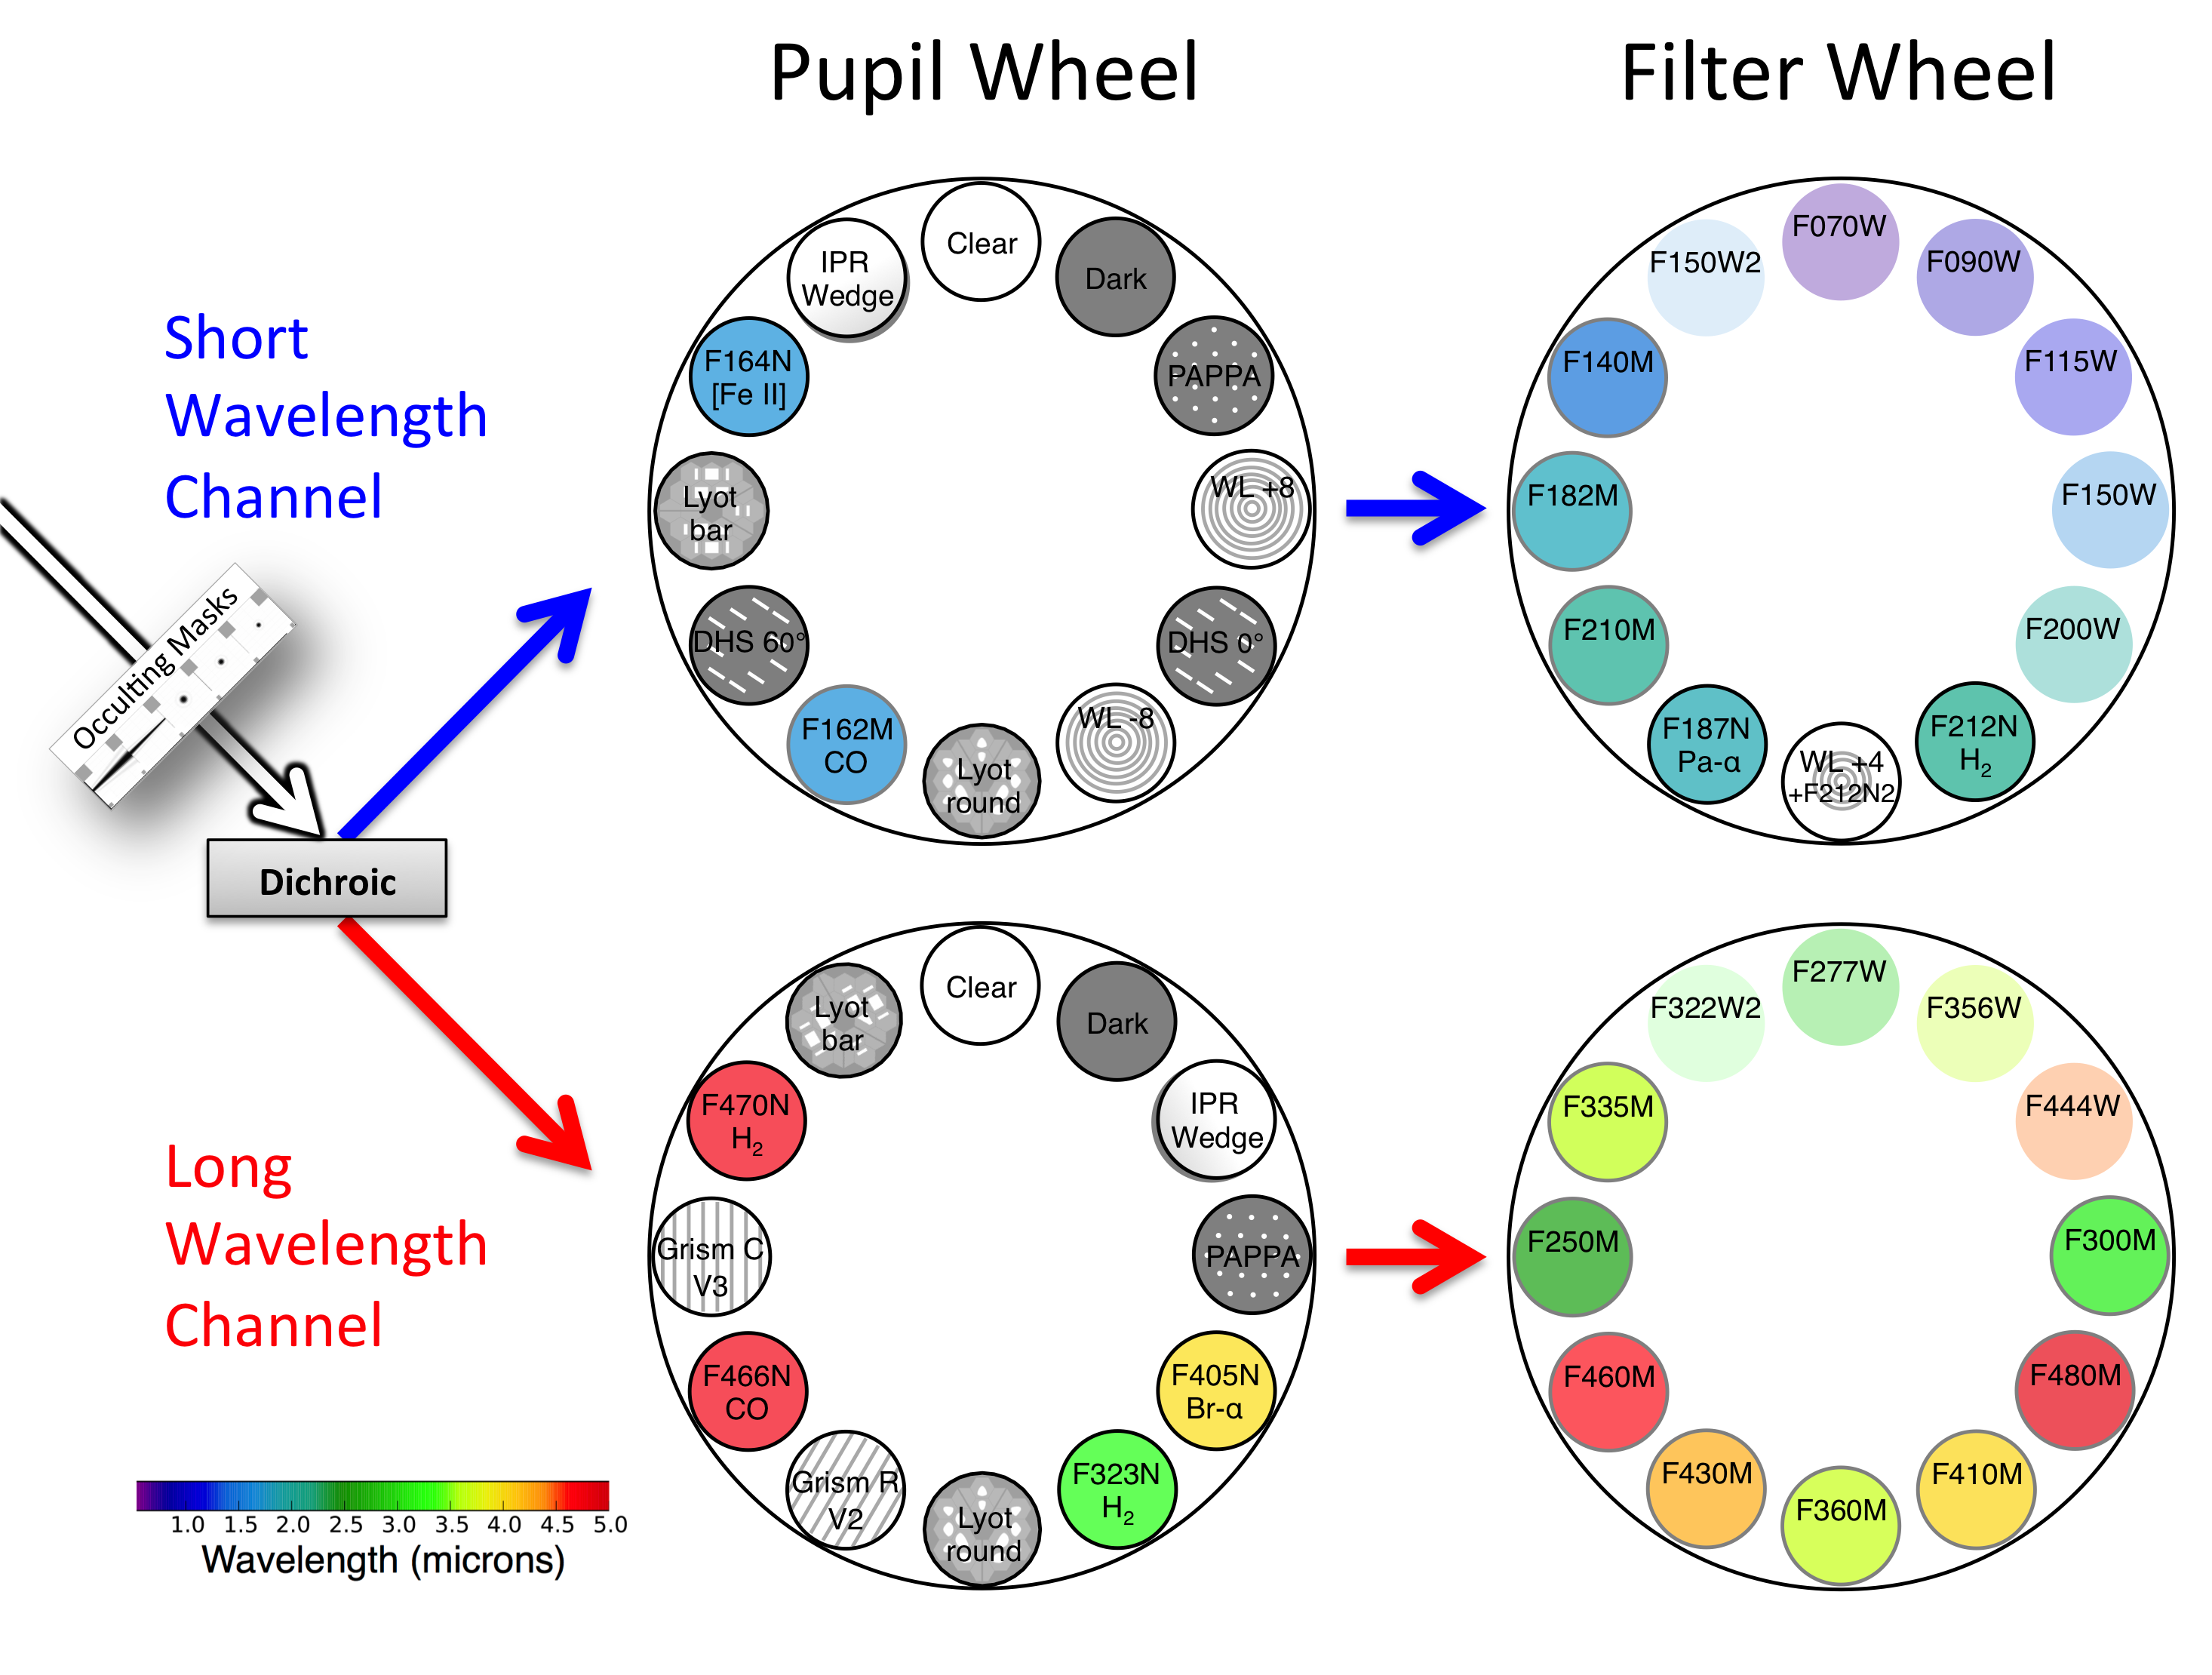
\includegraphics[scale=0.081]{wheels}
  \caption{Filter and pupil wheel configuration for NIRCam. Features two pairs of wheels: one pair for short wavelengths and one for longer wavelengths. Each pair has one wheel known as the `pupil' wheel which offers filters for different types of images, such as calibration or defocused light, and the `filter' wheel that primarily offers filters for different wavelengths of light \cite{webbwheels}.}
  \label{fig:wheels}
\end{figure}

\subsection{JWST Data Processing}
The processing of JWST goes through 4 stages. Stage 0 is raw data that is sent directly from JWST with zero processing or corrections. Stage 1 consists of detector-level corrections that are performed on a group-by-group basis. The output of this stage is a count rate image measuring the collection of photons.
Stage 2 includes additional instrument-level corrections to produce fully calibrated image exposures. There are different pipelines for imaging and spectroscopic exposures.

Stage 3 consists of working with multiple exposures and sometimes consists of combining exposures in some way \cite{webbstages}. 
This is the stage that is used in the project. Stage 3 processing adds corrections for astrometric alignment, background matching of the different mosaics, and outlier rejection \cite{webbstage3}. 
The output of this stage, for NIRCam imaging specifically, are (mostly) clean and calibrated images with metadata detailing photometry, physical positioning, timing, exposure, and much more.

\subsection{Post-Processing by Astronomers}
When the end goal is to output a color image from NIRCam, it is common that, using stage 3 data, several of the filter exposure images of a mission (i.e. a session of image captures that focus on one target object) are compiled in image processing software like Photoshop \cite{editinterview}. At this point, it is up to the graphics artist to interpret the exposures and try to output the most visually striking combination of filters using only three color channels.

\subsection{FITS File Format}
FITS files are the only format that house JWST (and most astronomical) data. All FITS files are composed of one or more header + data units (HDUs).
A header unit within one HDU consists of many records that make up something that resembles a standard dictionary data structure, but instead contains a key, value \emph{and} comment.

Alongside the header unit in an HDU, there may be an N-dimensional array, frequently a 1D spectrum, 2D image, or 3D data cube. The values in this array can be integers (signed, or unsigned for 8-bit), or floats of varying sizes \cite{fitsdoc}. This is the data unit of the HDU. Each FITS file can contain one or more of these HDUs.

In the context of JWST stage 3 data used in this project, it is very common that a FITS file contains a primary HDU that contains no data unit and a header unit with upwards of 300+ entries with information about the mission, target object, and previous stage's processing steps.

Alongside the primary HDU exists the ``science'' (SCI) HDU that contains the raw exposure data for a captured filtered exposure. The accompanying table of headers is a lot shorter and contains information regarding the applied filter(s), exposure time, spacecraft orientation, spatial extent, as well as other metadata pertinent to the capture of the image.

There are several other HDUs in the FITS file, most of which measure uncertainty and variance for each pixel in the SCI HDU data unit \cite{webbfits}. The remaining HDUs are currently not relevant to processing of the image data in this project.

Each FITS file corresponds to one captured filtered exposure.

\subsection{MAST}

The Mikulski Archive for Space Telescopes (MAST) is the sole repository that this project uses, and likely the only option to reliably retrieve JWST imaging data. Alongside JWST, MAST includes a wealth of datasets organized by ``collections'', from many missions, including ``HST, Kepler, GALEX, EUVE, FUSE, IUE, SWIFT, and several other missions'' \cite{mast}.

For each entry in MAST, there are several dozen metadata entries describing the image/data target, associated mission, time of capture, and more. For image and spectroscopy data, most data also comes with a preview image that comes in a widely viewable format like JPG.

Each mission will often have a handful of exposure captures in different wavelengths. Each of these has a different entry identifying the filters that were used. They are all under the same mission, target object name, and proposal ID. If one wanted to manually find all FITS files pertaining to one mission, they would need to search for a mission by one of those parameters and download each of the FITS files to get each filtered exposure used for that mission.

\subsection{Astropy and Python}
For this project, Python was used with several libraries including math and image processing libraries like NumPy, scikit-image, SciPy, and PIL. For astronomy related information processing, AstroPy, AstroQuery, and AstroAlign were also used. In this paper, the word ``script'' will be used to identify the program that was written for this project.

\section{Methodology}
\label{sec:script}
The general goal of this project was to acquire JWST imaging data automatically via script, process it in some way so that it becomes usable and recognizable to the viewer, then combine the all associated data in such a way that the output is a full color RGB image that is of the same quality as those released by the JWST team. This section will describe each step in the script that ultimately completes that goal.

\subsection{Data Acquisition}

The script that was created has two argument options to run. Choosing the argument \emph{query} will start the Query mode to allow the user to find a mission, and choosing the \emph{run} argument will allow the user to input a unique ID to automatically start the entire acquisition and processing pipeline.
\newline
\textbf{Query Mode:} On start, the user will be prompted with three search parameters: Name of the object, title of the mission, and proposal ID. Each of these prompts allow the user to narrow down search results of the future query output. If nothing is entered, all JWST data will be returned.

However, by default, there are several parameters that are applied that cannot be changed by the user. Therefore, the script is restricted to download data that matches each of the following criteria: it is JWST data, it is publicly available data, it is science (as opposed to measurement or calibration) data, it is a NIRCam image, and it is stage 3 data. Any additional parameters that the user initially entered are appended to this default list of parameters.

A query is then made to MAST using the aforementioned search parameters and a resulting CSV is written to the disk in an appropriate subdirectory.

The user will then need to search the CSV for the data that they seek and identify the proposal ID. The proposal ID is unique to each mission, and is short, making it a good unique identifier for a mission.
\newline
\textbf{Run Mode:} Upon starting run mode, the user will be prompted to enter a proposal ID. Upon entering the ID, MAST will be queried again, but this time to download all files relevant to that proposal's mission, and that conform to the aforementioned default search parameters.

The files will be downloaded to their own dedicated ``mission'' subdirectory. The FITS files for the mission will be sent to \emph{./missions/$<$target name$>$/data} and the preview of each FITS file will be sent to \emph{./missions/$<$target name$>$/preview}. Any future script executions of this same proposal ID will first check that the data already exists, and use existing data if possible. For the FITS files of the dataset used for this project, the total size on the disk was 2.27 GB.

Internally, after the files are either downloaded or read from the disk, the SCI HDU data unit image of each FITS file will be extracted and placed into an object that will also store metadata that is highly relevant to the image such as pixel size, spacecraft location and orientation, exposure time, and filters used. 
In case that there needs to be any processing of the image, this data can be readily accessed rather than opening the associated FITS file each time the information is needed. At this point, the images are ready to be processed.

\subsection{Managing the Pixel Values}
% value clip
The raw image data has a very high dynamic range: from just below zero (due to stage 1 or 2 calibration) all the way to 25,000 in one image. If these images were to be scaled down to between 0 and 255 without adjustment, only a speck of a star's corona would show up in the center of a black image.

A solution to allow detail to show up when scaled down would be to clip the values and ignore those that are simply too bright. I found that taking the 99.9\% highest value pixel as the new upper limit suffices (as well as taking the lower limit at 0). 
For all images in this project, the resulting highest values were in the double digits. When scaled to between 0 and 255, the detail is now very clear, and the clipping of star's extreme brightness is not noticeable. This clipping is applied to all images.

\subsection{Image Alignment}

Now that each image is of reasonable dynamic range, the next obvious issue is that each image has a different resolution. Additionally, not all images capture the same exact spatial extent in space. This is because each image is taken with a different filter, and each image is exposed for several minutes. Because there is movement onboard the telescope to swap filters with the filter wheel, the spacecraft's orientation is not consistent across all captures.

% bad alignment
The initial approach was to assume the images do indeed capture the same spatial extent. Therefore, a center focus pixel was needed in order to have a scaling origin for each image, which is available in the header unit of each image.

Next, each image needed to be scaled to the same nominal pixel area, then pad each image to they are indeed the same exact resolution. The result of this was was a failure on two fronts. First, while each image does come with a center X and center Y value, these values do not correspond to the same point in space, nor are they the exact center of the image. 
So, for the purposes of alignment, that statistic is useless. Second, each image does not cover the exact same spatial area, as mentioned previously. A new method was required to align the images in order to proceed.

% astroalign
I found the AstroAlign Python library does exactly what I needed. The primary alignment function required a ``target image'' and a ``source image'', where the source would be aligned to the target image. This function finds stars in the image and attempts to match the stars of the target image with the stars of the source image and derive a transformation that is then applied to the source image. The source image is then automatically cropped and padded to match the size of the target image.

After arbitrarily choosing a target image, the script attempts to align every  other image with the target. However, sometimes alignment with this method fails. If there is a failure, sensitivity and iteration parameters of the alignment function are adjusted and the alignment is retried. 
At some point, each image will either find an alignment, or fail once it is determined that alignment cannot be found. For the mission used in this project using only one target image, there are a resulting 4 images that share the same alignment: one target, and three successful alignments. The mission originally had 6 exposure images.

\subsection{Adding Color}
% turn to color
Now that there are a set of aligned images, the coloring process can start. The initial approach was to assign each filter to a color. This mapping can be seen as shifting infrared wavelengths band downward to the visible light spectrum such that the longest infrared will be mapped to red, and the shortest infrared wavelengths will be mapped to violet.

I created an array structure that would hold RGB values from 0 to 1 for several general bold colors sorted by wavelength: violet (1, 0, 0.5), blue (0, 0, 1), green (0, 1, 0), yellow (1, 1, 0) and red (1, 0, 0) to name a few. I then sorted the images based on their filter name. The filters have a naming convention that allows for them to be sorted alphabetically, resulting in them being ordered from shortest wavelength to longest. I then assigned each image to one of the color hues in an evenly-spaced fashion.

An RGB image is now made from each mono-color image where each channel is multiplied by the weights in the previously described color list. There are now 4 images that are colored from black to a color hue.

A second approach is to utilize the color assignment that the JWST team used. As it turns out, the color coding of filters in \cref{fig:filters} was carefully chosen, as it matches the idea that I originally had, but each filter has a corresponding color. I transcribed the colors chosen in the chart to a dictionary of filter names and RGB values, then simply created a color-hue image using those colors for each filter.

\subsection{Displaying the Image}

The final step was to combine the images in some way. After some experimenting with different methods, such add, blend, overlay, I found that the lighten operation yields the best results. Starting with a black image, the following algorithm is run: for each RGB channel of each image, take the maximum of the current image channel and the existing image's channel.

Finally, the resulting image is displayed, as well as saved to disk in 8-bit RGB format. Each major step's image result is also written to the disk in their own directories.

\section{Experiments}
\label{sec:exp}

Initial results of the script are promising, although there is certainly more that can be done, which will be addressed in \cref{sec:disc}.

\subsection{Success}

The final output of the script using the AstroAlign alignment method and the JWST team's color assignments yields an image (\cref{fig:output}) that is somewhat similar to the one that was publicly released of the same nebula target object (\cref{fig:original}). Immediately, it is easy to see some key differences. First, the outward orangish explosion is not visible in my image. This is because most of that color was in an image that was thrown out due to lack of usable alignment. 
Second, the blue color of the center of the nebula is not as vivid. There are two reasons for this: the green color image was also thrown out due to lack of usable alignment, and second, the publicly released image also goes through some post-processing to bring out color, simply for aesthetics.

\begin{figure}[t]
  \centering
  \includegraphics[scale=0.0494]{output}
  \caption{Final unedited output of my script. The color-to-filter mappings are: Blue = F090W; Cyan = F187N; Yellow = F356W; Red = F405N.}
  \label{fig:output}
\end{figure}

\subsection{Failures}

Before the final result in \cref{fig:output}, there were some failed attempts at alignment and coloring. As shown in \cref{fig:misaligned}, the shift in each color filter color channel is obvious. Since there are more color channels in use, the overall color looks different than my final correctly aligned one, despite using the same color assignment.

\begin{figure}[t]
  \centering
  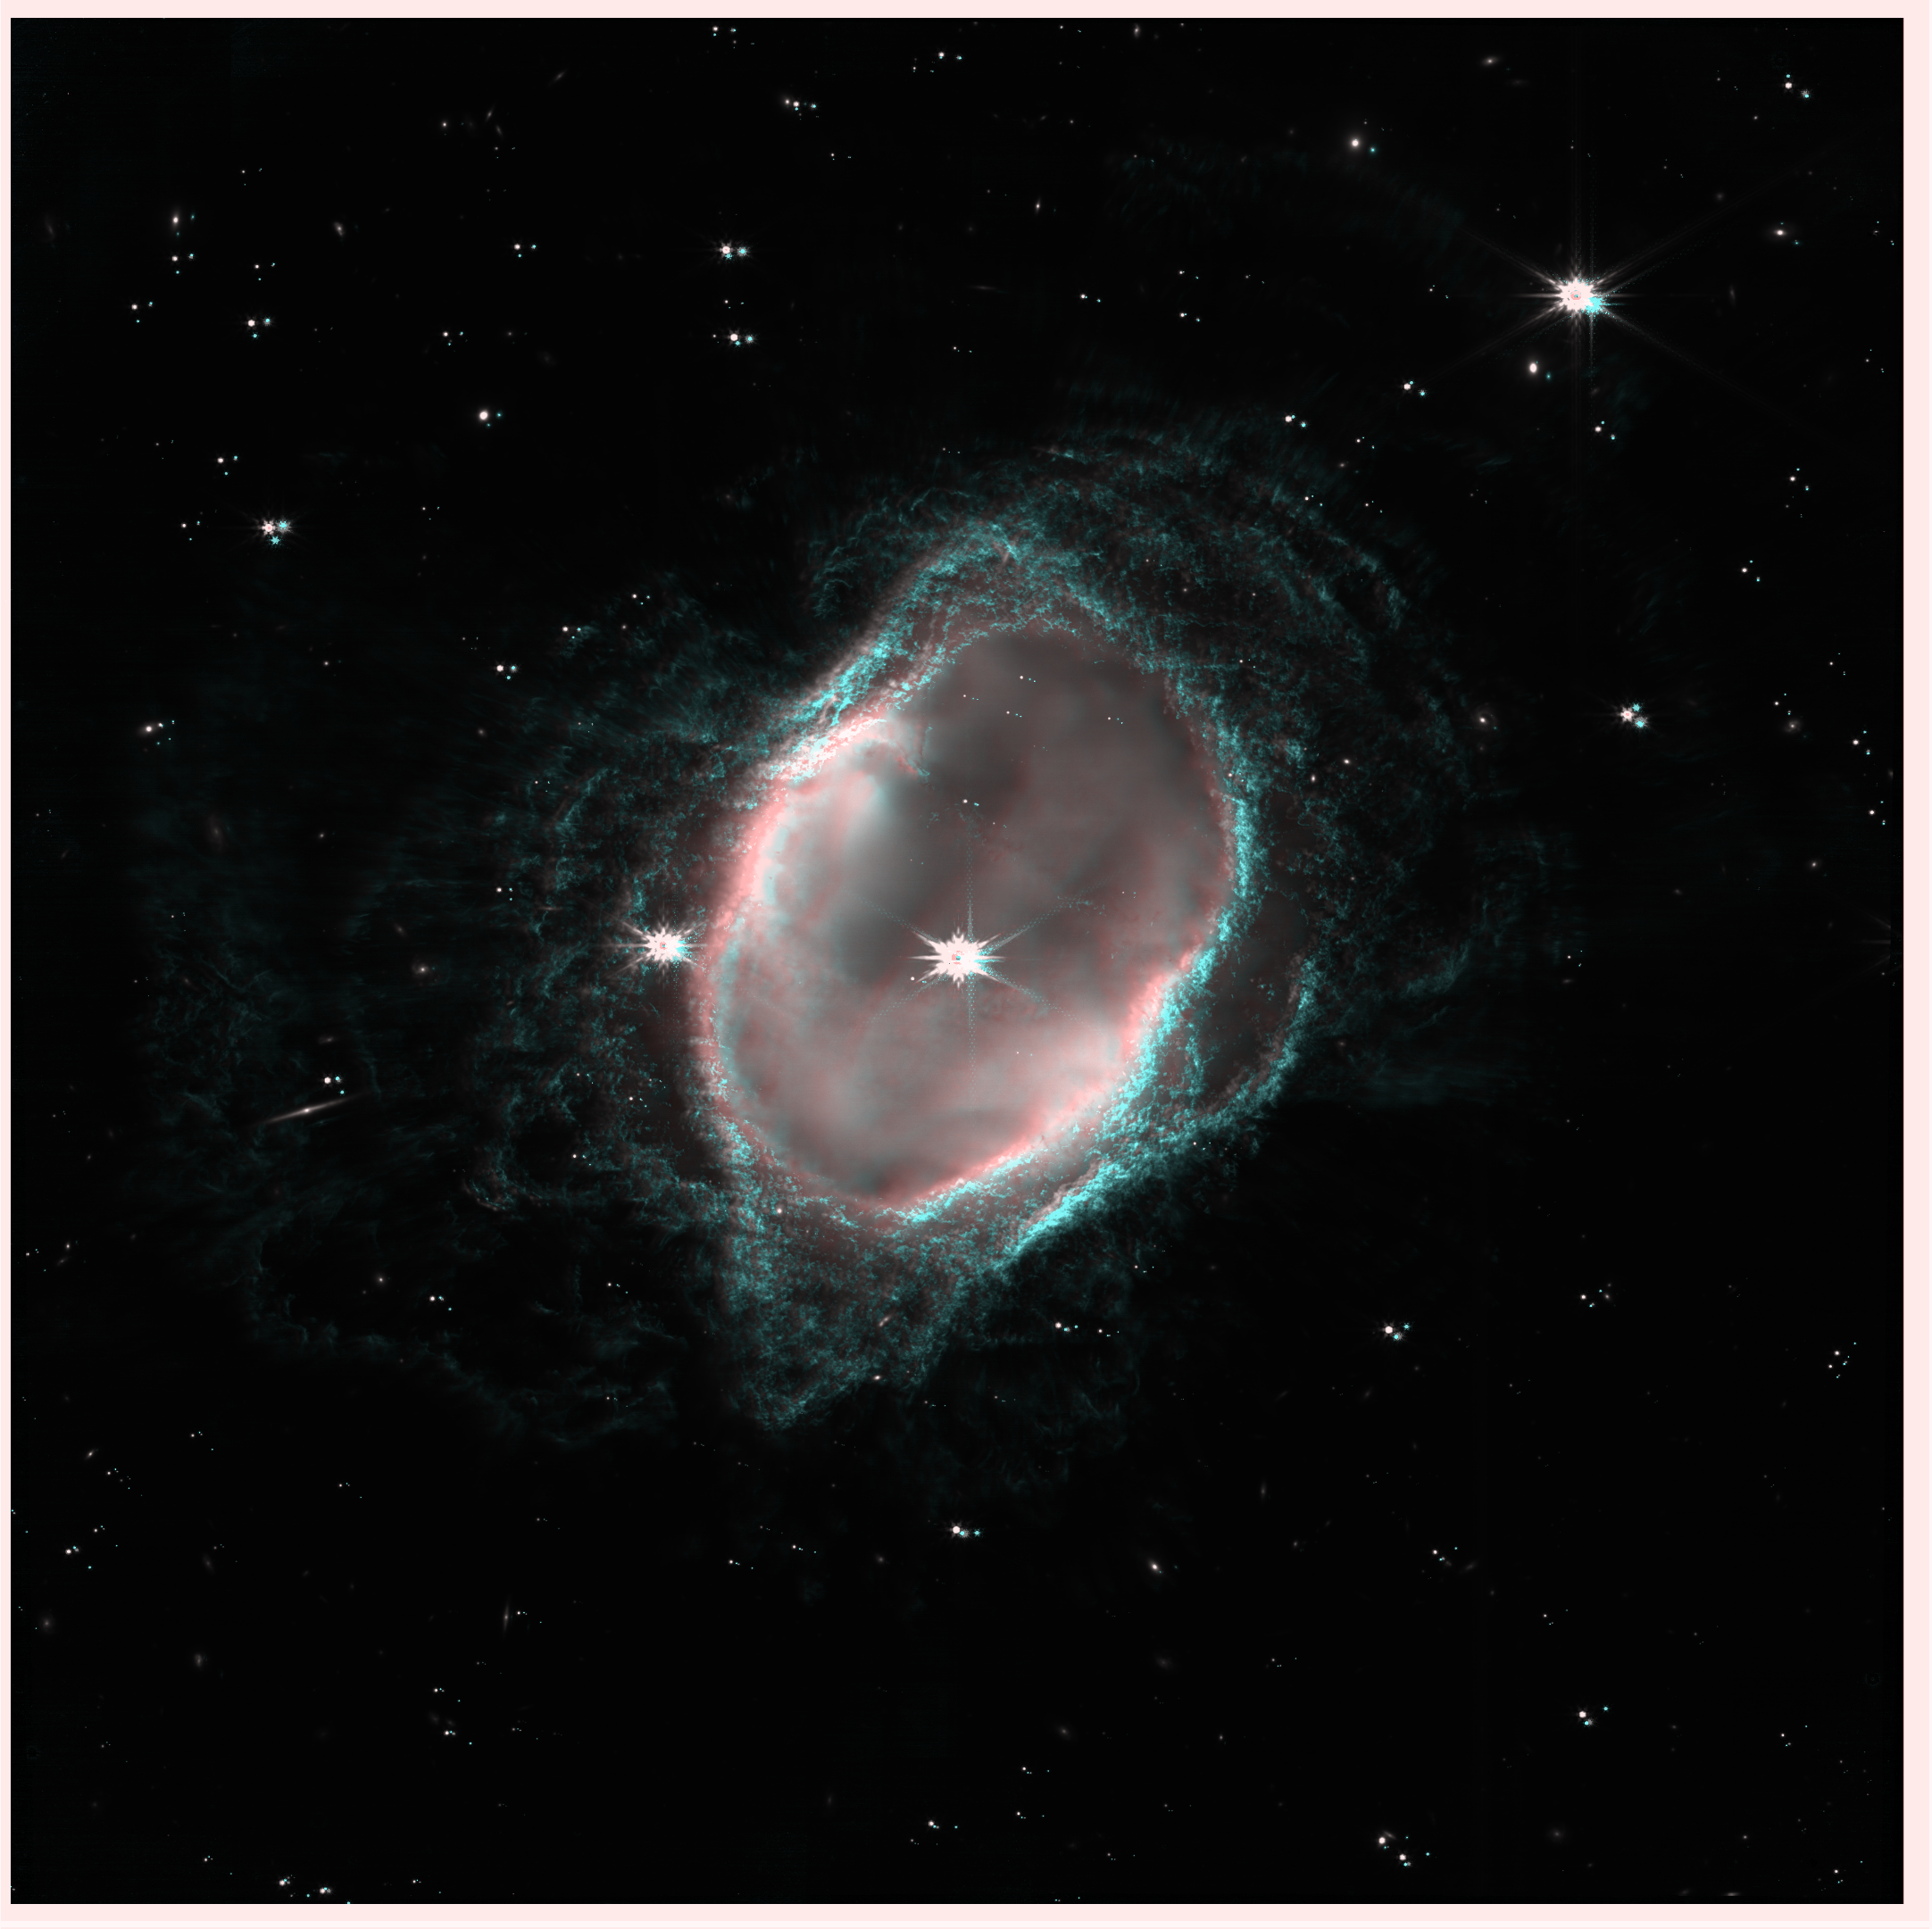
\includegraphics[scale=0.11]{misaligned2}
  \caption{Misaligned image with all available color filter images of my script. The color-to-filter mappings are:  Blue = F090W; Cyan = F187N; Green = F212N; Yellow = F356W; Red = F405N; Red = F470N.}
  \label{fig:misaligned}
\end{figure}

\begin{figure}[t]
  \centering
  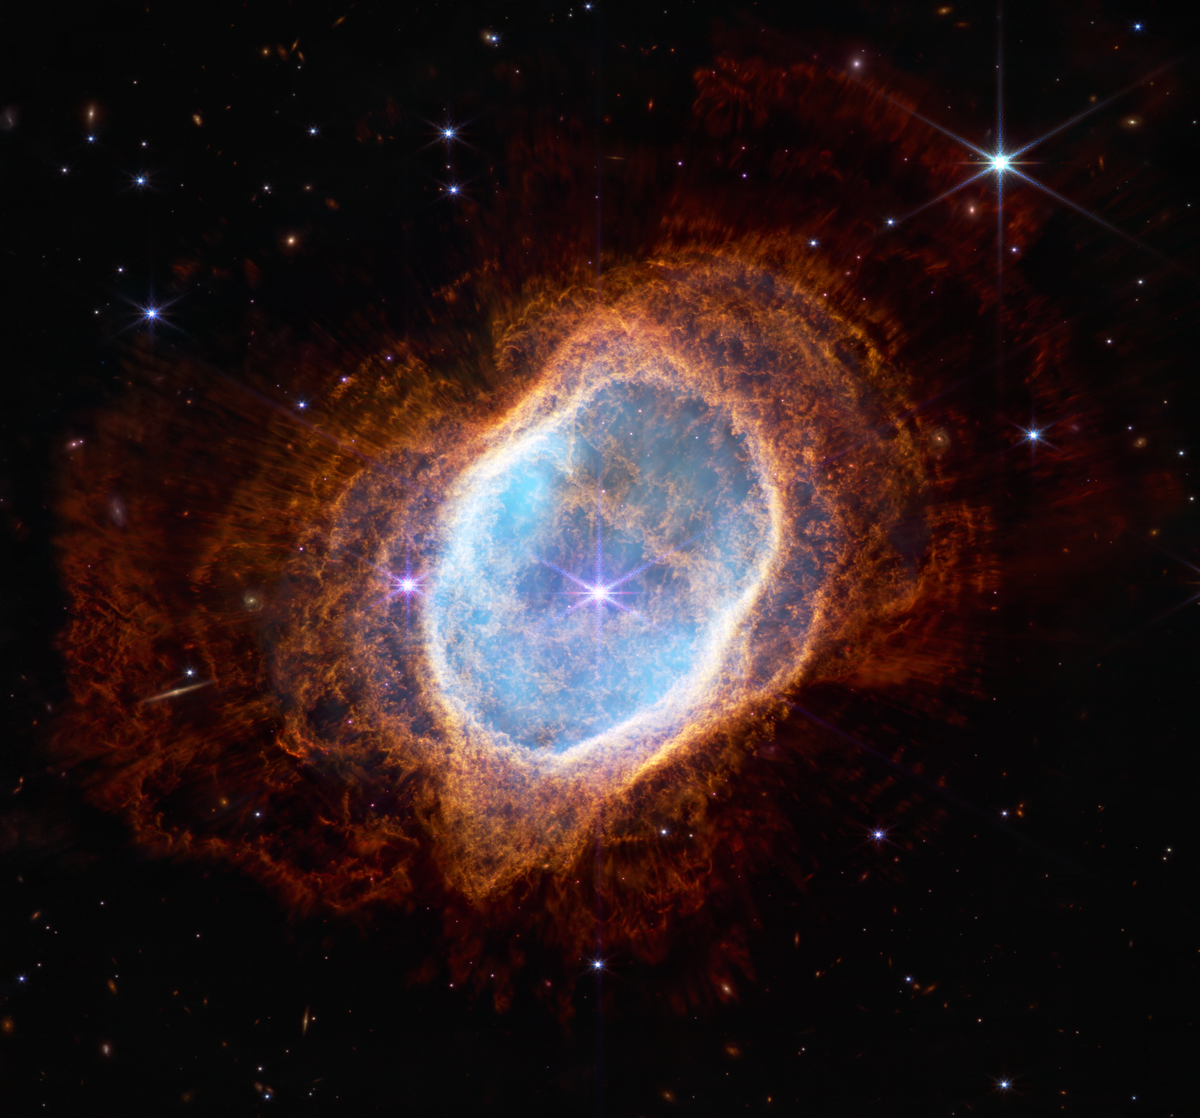
\includegraphics[scale=0.825]{wiki}
  \caption{Full color release image of NGC 3132 provided by NASA. The color-to-filter mappings are: Blue = F090W; Cyan = F187N; Green = F212N; Yellow = F356W; Red = F405N; Red = F470N.\cite{3132}}
  \label{fig:original}
\end{figure}

\section{Discussion}
\label{sec:disc}

Overall, this script and project were successful to an extent, but there is still a lot more that can be added to this script. If I had more time on this project, I would be able to attempt or complete a number of possible improvements.

\subsection{Occlusion Disc Flooding}

Firstly, a new feature that I did not attempt so far is a way to fill in the occluded spots. As mentioned when describing NIRCam, there is a way to occlude stars during image exposure. In the final color image result, a cyan circle and small black dot are visible in the center of the brightest stars in the image. 
During each exposure, the brightest parts are occluded, so when the images are combined, some channels are missing the full color of stars. This can be fixed by either flood-filling the 0-value pixels inside of a very high-value ``pit'' of pixel values, or waiting until the final color image is created before simply assigning the center of the stars to a full white color. Both of these approaches would require a method to find each occluded area, but the first would require this happening for each filter image, even if some are thrown out.

\subsection{Alignment}

A second improvement that can be made is the alignment. In the current script, the best alignment is done via AstroAlign. However, with this method, some of the images get dropped since no alignment can be found.

However, it might be possible to use that same function and achieve alignment with all images. If we were to choose a target image, we could build of images that align with that one. Then, we could assign those successfully-aligned images as the target, and try again on those that did not align the first time, and continue until all images are aligned. 
This method should work if the images failed to align due to a poor selection of target image. However, the primary downside to this method is that the runtime would be $O(n^2)$, where $n$ is the number of filter images. Since each $n$ can already take between 2-10 seconds, this alternative approach would significantly increase the runtime.

There are also other novel algorithms for alignment that could be investigated and implemented. However, one avenue that I have not fully explored is figuring out fully what each piece of image metadata is used for. For example, in each image, there is a spatial extent value. Paired with the spacecraft orientation and other values, a way to derive a transformation matrix may exist using already-known information.

\subsection{Color Assignment for Filters}

Another area that needs some exploring is the color assignment process. For the final image of this project, I used NASA's assignment. Since the source images are of wavelengths that are not visible to humans, the color selection is somewhat arbitrary. Realistically, I could develop my own equally-as-detailed color assignment that features more vivid and varied colors.

\subsection{Color Image Post-Processing}

Finally, as mentioned previously, the images released by NASA go through some post-processing in Photoshop to touchup and enhance the images for aesthetic purposes. Again, since these images are outside of our perception, it would not be unrealistic to programmatically enhance the final image result. 
A nice addition to this script would be a simple color curve adjustment. A simple curve adjustment done manually in a photo editor is visible in \cref{fig:enhancement}. A simple operation such as this could improve the aesthetics of the image, even with two missing filter images.

\begin{figure}[t]
  \centering
  \includegraphics[scale=0.066]{enhanced}
  \caption{The original aligned image plus minor color curve enhancement using paint.NET.}
  \label{fig:enhancement}
\end{figure}

\section{Conclusion}
\label{sec:conc}

The work done by NASA and the JWST team to publish the results of the telescope's data do a brilliant job of showing the beauty of the universe and garner interest in astronomy and astrophotography, and perhaps even gain support for JWST's mission. However, behind the vivid color images is a stack of raw data and several artists that manually create those color images.

The goal of this project was to attempt to automate some of the work that the artists do. This includes finding the images from the public archive, clipping, cropping, and stacking the images into perfectly aligned color images that illustrate the different wavelengths and physical makeup of celestial objects. 
The script that performs these actions does a great job of automatically acquiring the images, and an adequate job of clipping the images so their brightness is reasonable for a traditional 8-bit RGB image. As for combining the images using a simple merge operation, the script also does adequate work.

However, much work can still go into aligning the images and assigning colors to each layer. For alignment, it is quite possible that the same library that was used in this project can be used again, but at the cost of significant runtime increase. Alternatively, completely new algorithms can be used that may only take a fraction of the time. Or perhaps the wealth of metadata that comes with each image layer may hold all that is needed to align the images perfectly and in very little time.

As for image color assignment, it is important to know that the images that are captured from NIRCam are infrared; we as humans would not be able to see these images normally. Therefore, the assignment of colors to each image layer is technically subjective. Because of this, more research and trials could still go into finding the best-looking color assignment for each wavelength filter. 
Or, perhaps the best approach would be for the user of the script to choose the color assignment for each filter during runtime. This is the part of the project that leans more towards art than science.

Overall, given more time, a lot more could be added to this project. But given the allotted time, I would say this project was successful, and continuing this project may lead to even better results than those shown in this report.

\section{Project Source}
\label{sec:source}

The source code for this project is viewable via GitHub at \url{https://github.com/maxoakes/JWST-FITS-Reader}. After acquiring the handful of libraries required to run, one can easily run the script using the default settings to acquire the same images as the one in this report. It is recommended to have at least 2.5GB of free disk space before running.

\begin{thebibliography}{14}
\bibitem{webbobjective}
\referencelink{James Webb Space Telescope Science}{https://www.nasa.gov/mission_pages/webb/science/index.html}{Feb. 18, 2023}

\bibitem{webbtools}
\referencelink{JWST Missions and Data}{https://archive.stsci.edu/missions-and-data/jwst}{Jan 11, 2023}

\bibitem{webbmiri}
\referencelink{MIRI Imaging - JWST User Documentation}{https://jwst-docs.stsci.edu/jwst-mid-infrared-instrument/miri-observing-modes/miri-imaging}{Feb. 18, 2023}

\bibitem{webbnircam}
\referencelink{JWST Near Infrared Camera - JWST User Documentation}{https://jwst-docs.stsci.edu/jwst-near-infrared-camera}{Feb. 18, 2023}

\bibitem{webbniriss}
\referencelink{NIRISS Imaging - JWST User Documentation}{https://jwst-docs.stsci.edu/jwst-near-infrared-imager-and-slitless-spectrograph/niriss-observing-modes/niriss-imaging}{Feb. 18, 2023}

\bibitem{webbnirspec}
\referencelink{JWST Near Infrared Spectrograph - JWST User Documentation}{https://jwst-docs.stsci.edu/jwst-near-infrared-spectrograph}{Feb. 18, 2023}

\bibitem{webbfilters}
\referencelink{NIRCam Filters - JWST User Documentation}{https://jwst-docs.stsci.edu/jwst-near-infrared-camera/nircam-instrumentation/nircam-filters}{Feb. 10, 2023}

\bibitem{webbwheels}
\referencelink{NIRCam Pupil and Filter Wheels - JWST User Documentation}{https://jwst-docs.stsci.edu/jwst-near-infrared-camera/nircam-instrumentation/nircam-pupil-and-filter-wheels}{Mar 23, 2023}

\bibitem{webbstages}
\referencelink{Pipeline Stages}{https://jwst-pipeline.readthedocs.io/en/stable/jwst/pipeline/main.html}{Jan 20, 2023}

\bibitem{webbstage3}
\referencelink{calwebb image3: Stage 3 Imaging Processing}{https://jwst-pipeline.readthedocs.io/en/stable/jwst/pipeline/calwebb_image3.html}{Jan 20, 2023}

\bibitem{editinterview}
\referencelink{Here's how to edit James Webb Space Telescope images}{https://www.space.com/james-webb-space-telescope-image-editing}{Feb 18, 2023}

\bibitem{fitsdoc}
\referencelink{Flexible Image Transport System (FITS), Version 3.0}{https://www.loc.gov/preservation/digital/formats/fdd/fdd000317.shtml}{Jan 20, 2023}

\bibitem{webbfits}
\referencelink{Calibrated data: cal and calints}{https://jwst-pipeline.readthedocs.io/en/stable/jwst/data_products/science_products.html\#calibrated-data-cal-and-calints}{Jan 20, 2023}

\bibitem{mast}
\referencelink{MAST: Barbara A. Mikulski Archive for Space Telescopes}{https://mast.stsci.edu/portal/Mashup/Clients/Mast/Portal.html}{Jan 11, 2023}

\bibitem{3132}
\referencelink{NASA's Webb Captures Dying Star's Final `Performance' in Fine Detail}{https://webbtelescope.org/contents/news-releases/2022/news-2022-033}{March 21, 2023}

\end{thebibliography}

\end{document}